\documentclass[11pt]{article}

\usepackage{listings}
\usepackage{epsfig}
\usepackage{lscape}
\usepackage{multirow}
\usepackage{longtable}
\usepackage{amsmath,amssymb,amsthm}
\usepackage{graphicx}
\usepackage{color}
\usepackage{placeins}
\usepackage{url}
\usepackage{cases}
\usepackage{hyperref}
\usepackage{setspace}
\usepackage{subfigure}
\usepackage{float}
\usepackage{listings}
\usepackage{framed}
\usepackage[c2]{optidef}
\usepackage{tikz}
\usepackage{caption}
\usepackage{algorithm}
\usepackage{algorithmic}
\usepackage{endnotes}


\usepackage{booktabs}

\oddsidemargin 0pt
\evensidemargin 0pt
\marginparwidth 10pt
\marginparsep 10pt
\topmargin -20pt
\textwidth 6.5in
\textheight 8.5in
\parindent = 20pt

\DeclareMathOperator*{\argmin}{argmin}
\DeclareMathOperator*{\minimax}{minimax}

\renewcommand{\algorithmicrequire}{ \textbf{function:}}
\renewcommand{\algorithmicreturn}{ \textbf{end function}}
\newcommand{\blue}[1]{\begin{color}{blue}#1\end{color}}
\newcommand{\magenta}[1]{\begin{color}{magenta}#1\end{color}}
\newcommand{\red}[1]{\begin{color}{red}#1\end{color}}
\newcommand{\green}[1]{\begin{color}{green}#1\end{color}}

\newtheorem{theorem}{Theorem}
\newtheorem{proposition}{Proposition}
\newtheorem{lemma}{Lemma}
\newtheorem{corollary}{Corollary}
\newtheorem{remark}{Remark}
\newtheorem{assumption}{Assumption}
\newtheorem{definition}{Definition}
%\newenvironment{proof}{{\noindent\it Proof}\quad}{\hfill $\square$\par}

%\usepackage{sidecap}


\begin{document}
	
	\title{\bf Project Report}
	
	\author{Boyuan Yao 19307110202}
	
	
	\date{\today}
	\maketitle

\section{Introduction}
	I gained inspiration from a paper "poisson image editing" by P\'erez $\left[1\right]$. Solving a poisson equation, this method can simply insert part of sources image into the target one, which can cover the case that drastic differences between the souces and destination exist. Moreover, with appropriate modifying of the so called \textit{guidance filed}, we could even retain the feature of the background of target image, that is to say we could insert some transparant sources into the destination. In the second sector, I'm going to show the basic idea of this method. In the third sector, I'll show several experiments using the FDM. We will see a fourier approximation approach to solve the poisson equation in the fourth section, which is included in the work of J. Mat\'ias Di Martino$\left[2\right]$. I will give two brief pseudocodes in the last section.

\section{Basic idea}
	
	\begin{figure}[H]
		\centering
		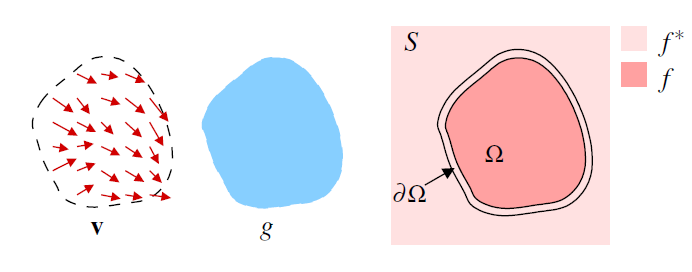
\includegraphics[scale=0.9]{figure1.png}
		\caption{\textbf{Guided interpolation notations.} Unknown function $f$ interpolates in domain $\Omega$ the destination function $f^*$, under guidance field $\boldsymbol{v}$ \protect \footnotemark[1]}
	\end{figure}
	\footnotetext[1]{P. P\'erez, M. Gangnet, and A. Blake, \textit{Poisson image editing}, ACM Transactions on Graphics, 22 (2003), p.314.}
	The basic idea of the approach is to interpolate the destination function $f^*$ on a subdomain $\Omega$ with an unkown function $f$. The simplest interpolant $f$ of $f^*$ is called membrane interpolant, it is the solution of the minimization problem:
	\begin{equation}
		\min\limits_f \iint_{\Omega}^{} |\nabla f|^2 \quad \text{s.t.} \quad f|_{\partial \Omega} = f^*|_{\partial \Omega}
	\end{equation}
	The solution of problem (1) is:
	
	\begin{equation}
		\Delta f|_\Omega = 0 \quad \text{with} \quad f|_{\partial \Omega} = f^*|_{\partial \Omega}
	\end{equation}
	If a \textit{guidance field} $\boldsymbol{v}$ is given, the problem (1) could be extended as
	
	\begin{equation}
		\min\limits_f \iint_{\Omega}^{} |\nabla f - \boldsymbol{v}|^2 \quad \text{s.t.} \quad f|_{\partial \Omega} = f^*|_{\partial \Omega}
	\end{equation}
	Then the solution is
	
	\begin{equation}
		\Delta f|_{\Omega} = \text{div} \boldsymbol{v} \quad \text{with} \quad f|_{\partial \Omega} = f^*|_{\partial \Omega}
	\end{equation}
	Where $\text{div} \boldsymbol{v} = \frac{\partial u}{\partial x} + \frac{\partial v}{\partial y}$ is the divergence of $\boldsymbol{v} = (u,v)$. Therefore, the interpolation problem could be converted into a poisson function with Dirichlet boundary condition.
	~\\
	Then back to the problem we focus, in the poisson image editing, the \textit{guidance field} is given by calculating the gradient of the part of sources image that is to be inserted into the target one together with the destination domain, and the boundary condition could be attained from the target image. I implement two types of Seamless cloning in my project, with importing gradients and mixing gradients.
	
\subsection{Importing gradients}
	Importing gradients is a basic choice for the \textit{guidance field}, which has the following form
	
	\begin{equation}
		\boldsymbol{v} = \nabla g
	\end{equation}
	Where $g$ denotes the source image, then problem (4) could be presented by this
	
	\begin{equation}
		\Delta f|_{\Omega} = \Delta g \quad \text{with} \quad f|_{\partial \Omega} = f^*|_{\partial \Omega}
	\end{equation}
	With the above equations, we are able to insert the source image into the target image seaminglessly. But notice that in the domain $\Omega$, the information of gradient of the background image has been completely replaced by the source image, we can not hold the properties of target image inside the domain. The shortcoming of the improting gradients implementation will display when you want to insert a transparent item or you want to hold the texture of the background image to some degree. To solve this, we have the following implementation called mixing gradients.
	

	
\subsection{Mixing gradients}
	In this part we simply reformulate the \textit{guidance field} like this
	
	\begin{equation}
		\boldsymbol{v} = 
		\begin{cases}
			\nabla f^* & ||\nabla f^*|| > ||\nabla g|| \\
			\nabla g & \text{Otherwise}
		\end{cases}
	\end{equation} 
	With the above reformulation, we are able to insert some transparent items into the destination image or stop the object in the target image bleeds into the domain when they are close enough.
	
\section{Finite Difference Method}
	
	To solve the given poisson equation, I first implement a solver using finite difference method to solve the discretization poisson equation. With Gaussian Seidel iteration, it could solve some of the problem with small cases, but works slowly when the number of pixels growth to certain degree. The followings are some results of my experiments.

	\begin{figure}[H]
		\centering
		\subfigure[source]{
			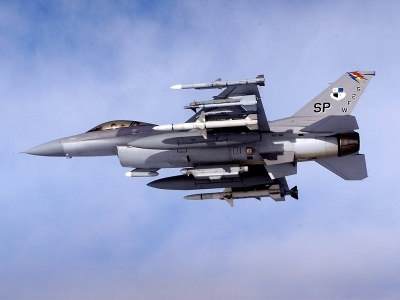
\includegraphics[scale=0.2]{demo2_sources.jpg}
		}
		\subfigure[mask]{
			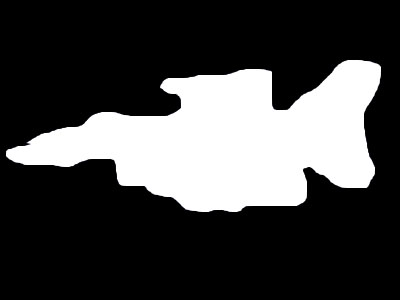
\includegraphics[scale = 0.2]{demo2_mask.jpg}
		}
		\subfigure[target]{
			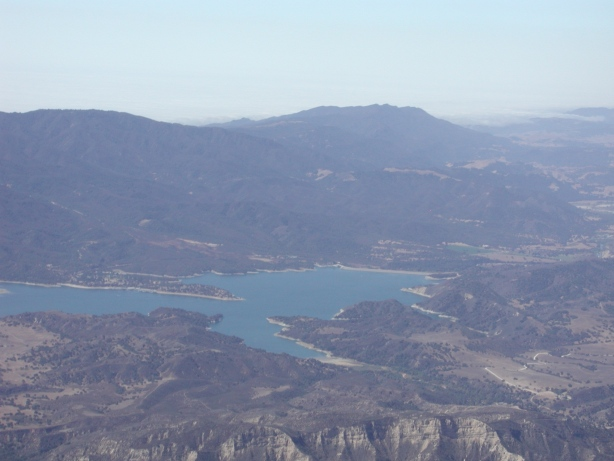
\includegraphics[scale = 0.2]{demo2_target.jpg}
		}
		\subfigure[outcome]{
			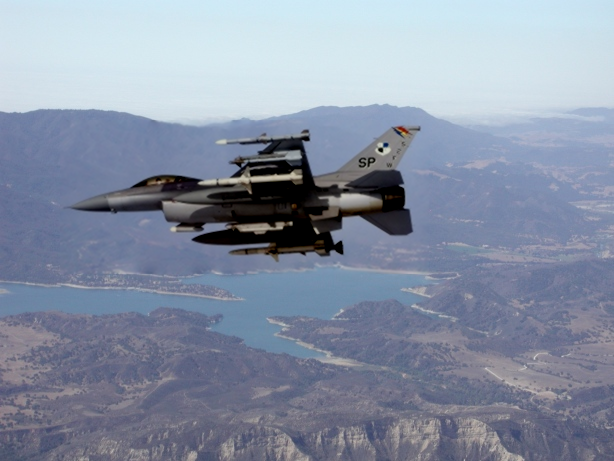
\includegraphics[scale = 0.2]{demo2_outcome.png}
		}
		\caption{Importing gradients\protect\footnotemark[2]}
	\end{figure}
	\footnotetext[2]{Some of the pictures are from http://cs.brown.edu/courses/csci1950-g/results/proj2/pdoran/}
	\begin{figure}[H]
		\centering
		\subfigure[source]{
			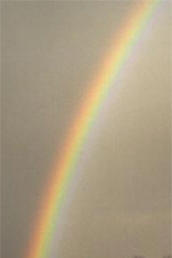
\includegraphics[scale=3]{demo5_sources.jpg}
		}
		\subfigure[mask]{
			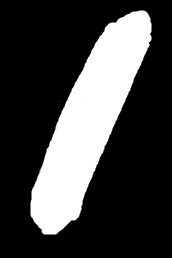
\includegraphics[scale=3]{demo5_mask.jpg}
		}
		\subfigure[target]{
			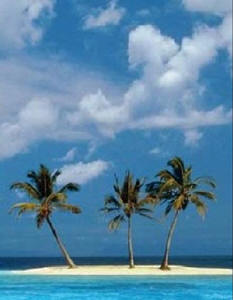
\includegraphics[scale=3]{demo5_target.jpg}
		}
		\subfigure[importing gradients]{
			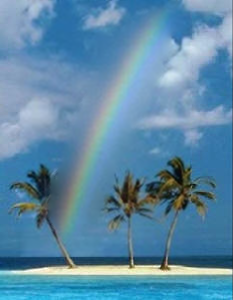
\includegraphics[scale=0.45]{demo5_outcome.png}
		}
		\subfigure[mixing gradients]{
			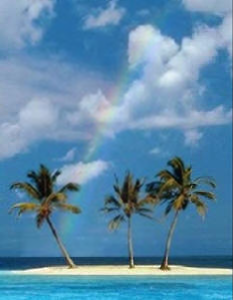
\includegraphics[scale=0.45]{demo5_mixed_outcome.png}
		}
		\caption{\textbf{Importing gradients vs Mixing gradients} We could see from the experiments above that when inserting an transparent object into the destination mixing gradients performes better than simply importing gradients}
	\end{figure}
	\begin{figure}[H]
		\centering
		\subfigure[source]{
			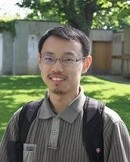
\includegraphics[scale=0.6]{demo4_sources.jpg}
		}
		\subfigure[mask]{
			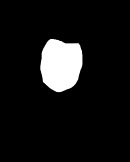
\includegraphics[scale = 0.6]{demo4_mask.jpg}
		}
		\subfigure[target]{
			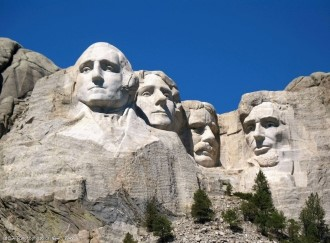
\includegraphics[scale = 0.6]{demo4_target.jpg}
		}
		\subfigure[outcome]{
			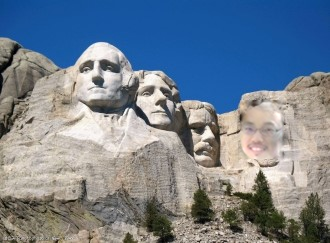
\includegraphics[scale = 0.45]{demo4_outcome.png}
		}
	
		\subfigure[source]{
			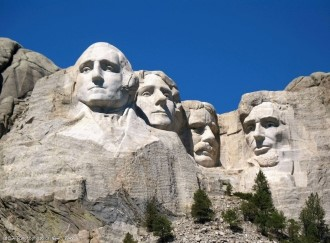
\includegraphics[scale=0.6]{demo7_sources.jpg}
		}
		\subfigure[mask]{
			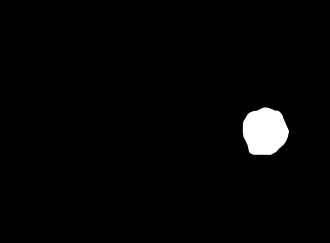
\includegraphics[scale = 0.6]{demo7_mask.jpg}
		}
		\subfigure[target]{
			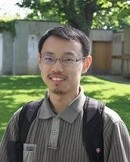
\includegraphics[scale = 0.6]{demo7_target.jpg}
		}
		\subfigure[outcome]{
			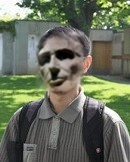
\includegraphics[scale = 0.45]{demo7_outcome.png}
		}
		\caption{A funny case, just enjoy!}
	\end{figure}
	
\section[Fourier Approach]{Fourier Approach \footnote[3]{J. Mat\'ias Di Martino, Gabriele Facciolo, Enric Meinhardt-Llois, \textit{Poisson Image Editing}, Image Processing On Line, 6 (2016), p.309-311.}}
	
	To work on the problem using Fourier approach, we first need to transform the original problem (1) into the following approximation problem
	
	\begin{equation}
		\Delta f|_S = \text{div} \boldsymbol{V} \quad \text{with} \quad \nabla f \cdot \nu |_{\partial S} = 0
	\end{equation}
	As we solve the problem on the entire domain $S$, the \textit{guidance field} $\boldsymbol{V}$ has the following form
	
	\begin{equation}
		V = 
		\begin{cases}
			v & \text{in domain} \Omega\\
			\nabla f^* & \text{Otherwise}
		\end{cases}
	\end{equation}
	
	To use the Fourier approach, we should first consider the discrete bidimentional Fourier transformation of 2-D signal $Z$ with size $H \times W$
	
	\begin{equation}
		\hat{Z}(u,v) = \sum\limits_{x = 0}^{W - 1}\sum\limits_{y = 0}^{H - 1} Z(x,y)e^{-2\pi i (\frac{xu}{W} + \frac{yv}{H})}
	\end{equation}
	and its inverse,
	
	\begin{equation}
		Z(x,y) = \frac{1}{WH} \sum_{u = 0}^{W - 1}\sum_{v = 0}^{H - 1}\hat{Z}(u,v)e^{2\pi i (\frac{xu}{W} + \frac{yv}{H})}
	\end{equation}
	Therefore the DFT has the following properties
	
	\begin{equation}
		\frac{\widehat{\partial Z}}{\partial x} = \frac{2 \pi i}{W} u \hat{Z}, \frac{\widehat{\partial Z}}{\partial y} = \frac{2 \pi i}{H} v \hat{Z}
	\end{equation}
	Then we are able to convert the problem (8) into the following form
	
	\begin{equation}
		\left[(\frac{2\pi i}{W})^2 u^2 + (\frac{2\pi i}{H})^2 v^2\right]\hat{f}_{uv} = \frac{2 \pi i}{W} u \widehat{V^x}_{uv} + \frac{2 \pi i}{H} v \widehat{V^y}_{uv}
	\end{equation}
	Where $\widehat{V^x},\widehat{V^y}$ denotes the partial derivatives of field $\boldsymbol{V}$. When $u = v = 0$, we could simply let $\hat{f}_{uv} = 0$, cause zero frequency just influence the solution by a constant value. After calculating the inverse of $\hat{f}$, we apply a shift of the solution to recover the color and the brightness of the image. Moreover, to hold the Neumann boundary conditions $\nabla f \cdot \nu |_{\partial S} = 0$, we could extend the input gradient field $\boldsymbol{V}$ so that the components $V^x$ and $V^y$ are antisymmetric with respect to $x$ and $y$ axis respectively. Then we have extended gradient fields which are four times bigger and become symmetric and periodic. After solving the reformulated system, we restrict the solution to the original domain and attain the solution we want. The details could be found in the source code of my project.
	~\\
	This approach is much faster than FDM written by myself. With the aid of this approach I am able to implement poisson image editing on images with higher quality(more pixels). The followings are some of my results.
	
	\begin{figure}[H]
		\centering
		\subfigure[source]{
			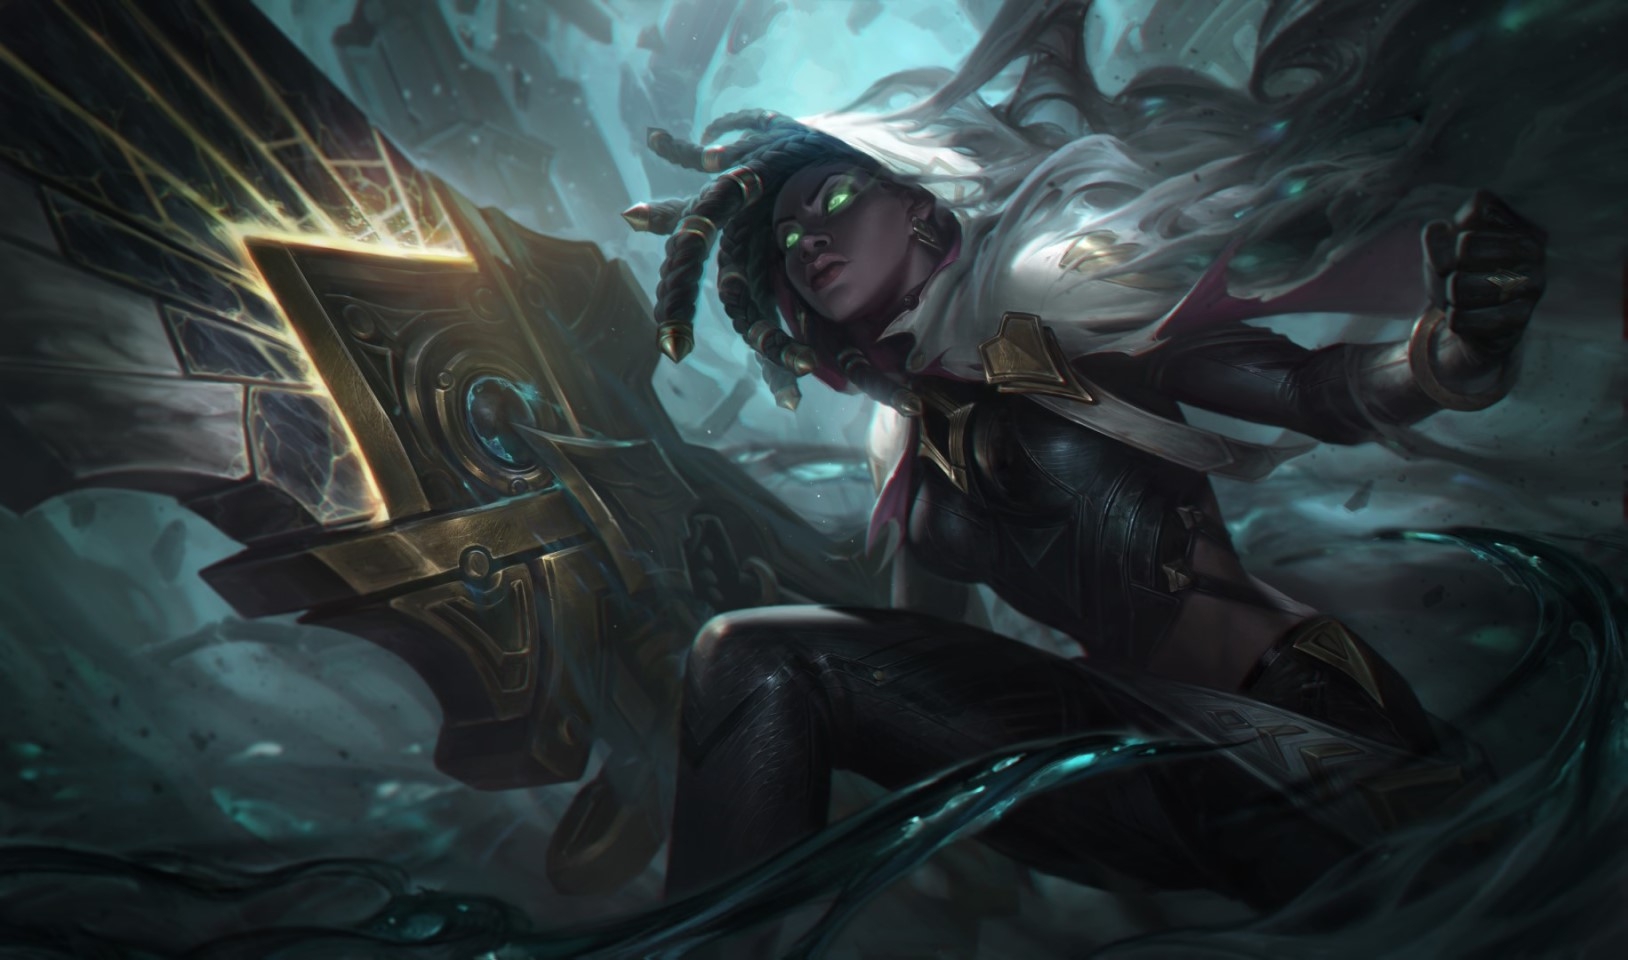
\includegraphics[scale=0.1]{demo1_sources_FFT.jpg}
		}
		\subfigure[mask]{
			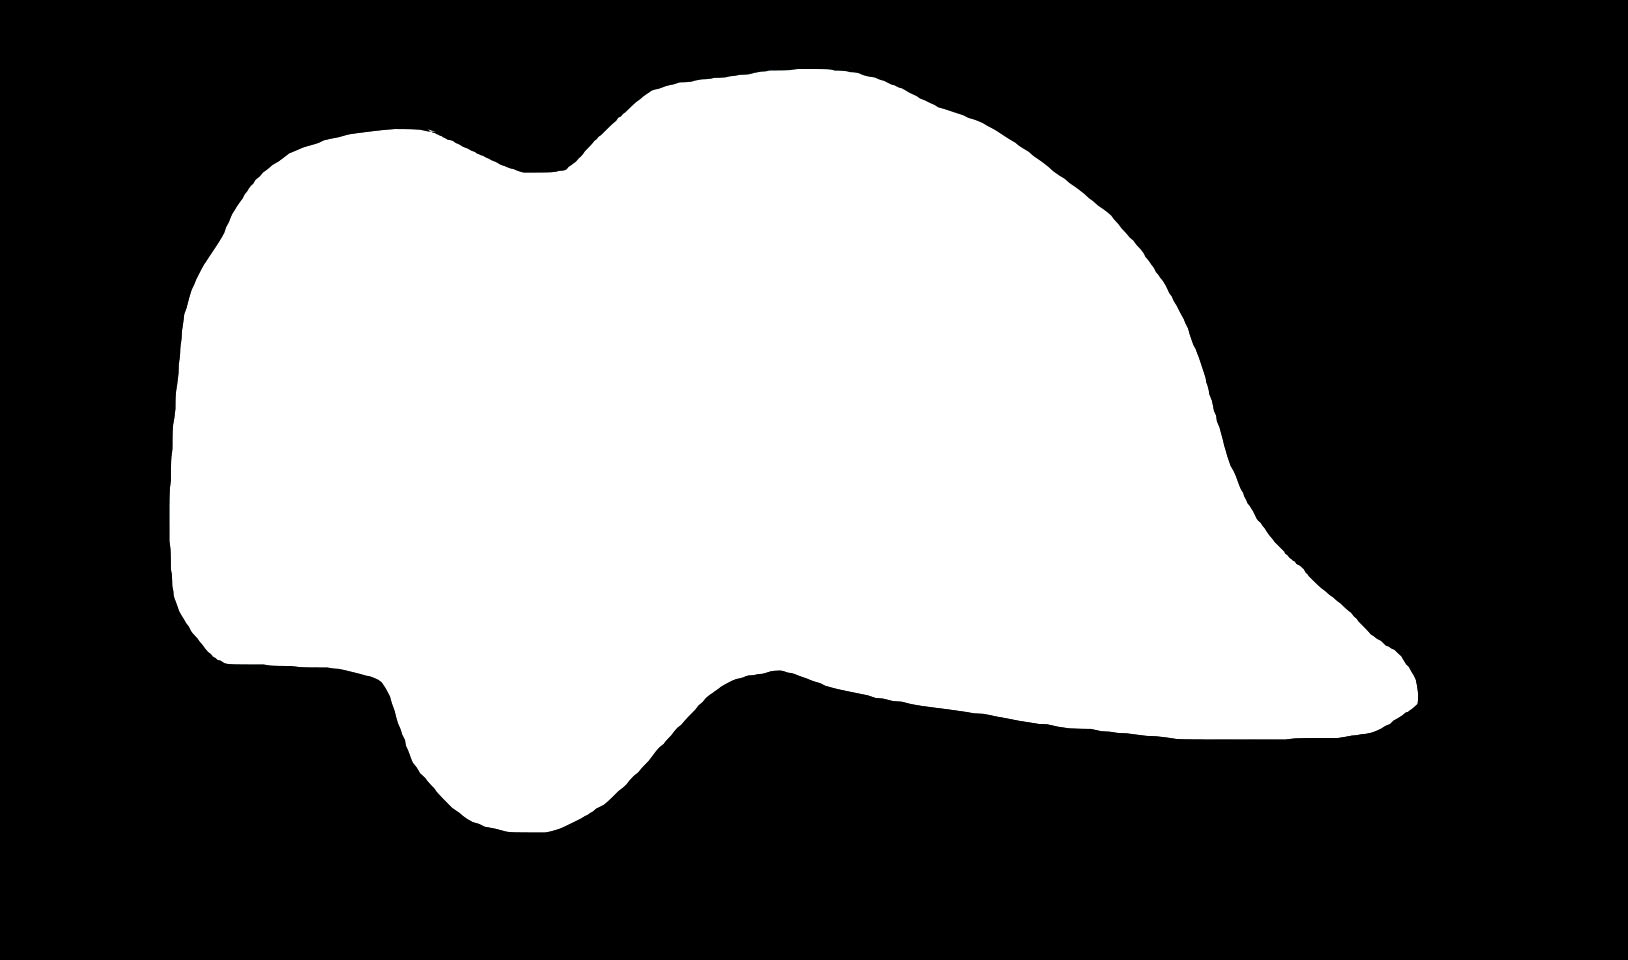
\includegraphics[scale = 0.1]{demo1_mask_FFT.jpg}
		}
	
		\subfigure[target]{
			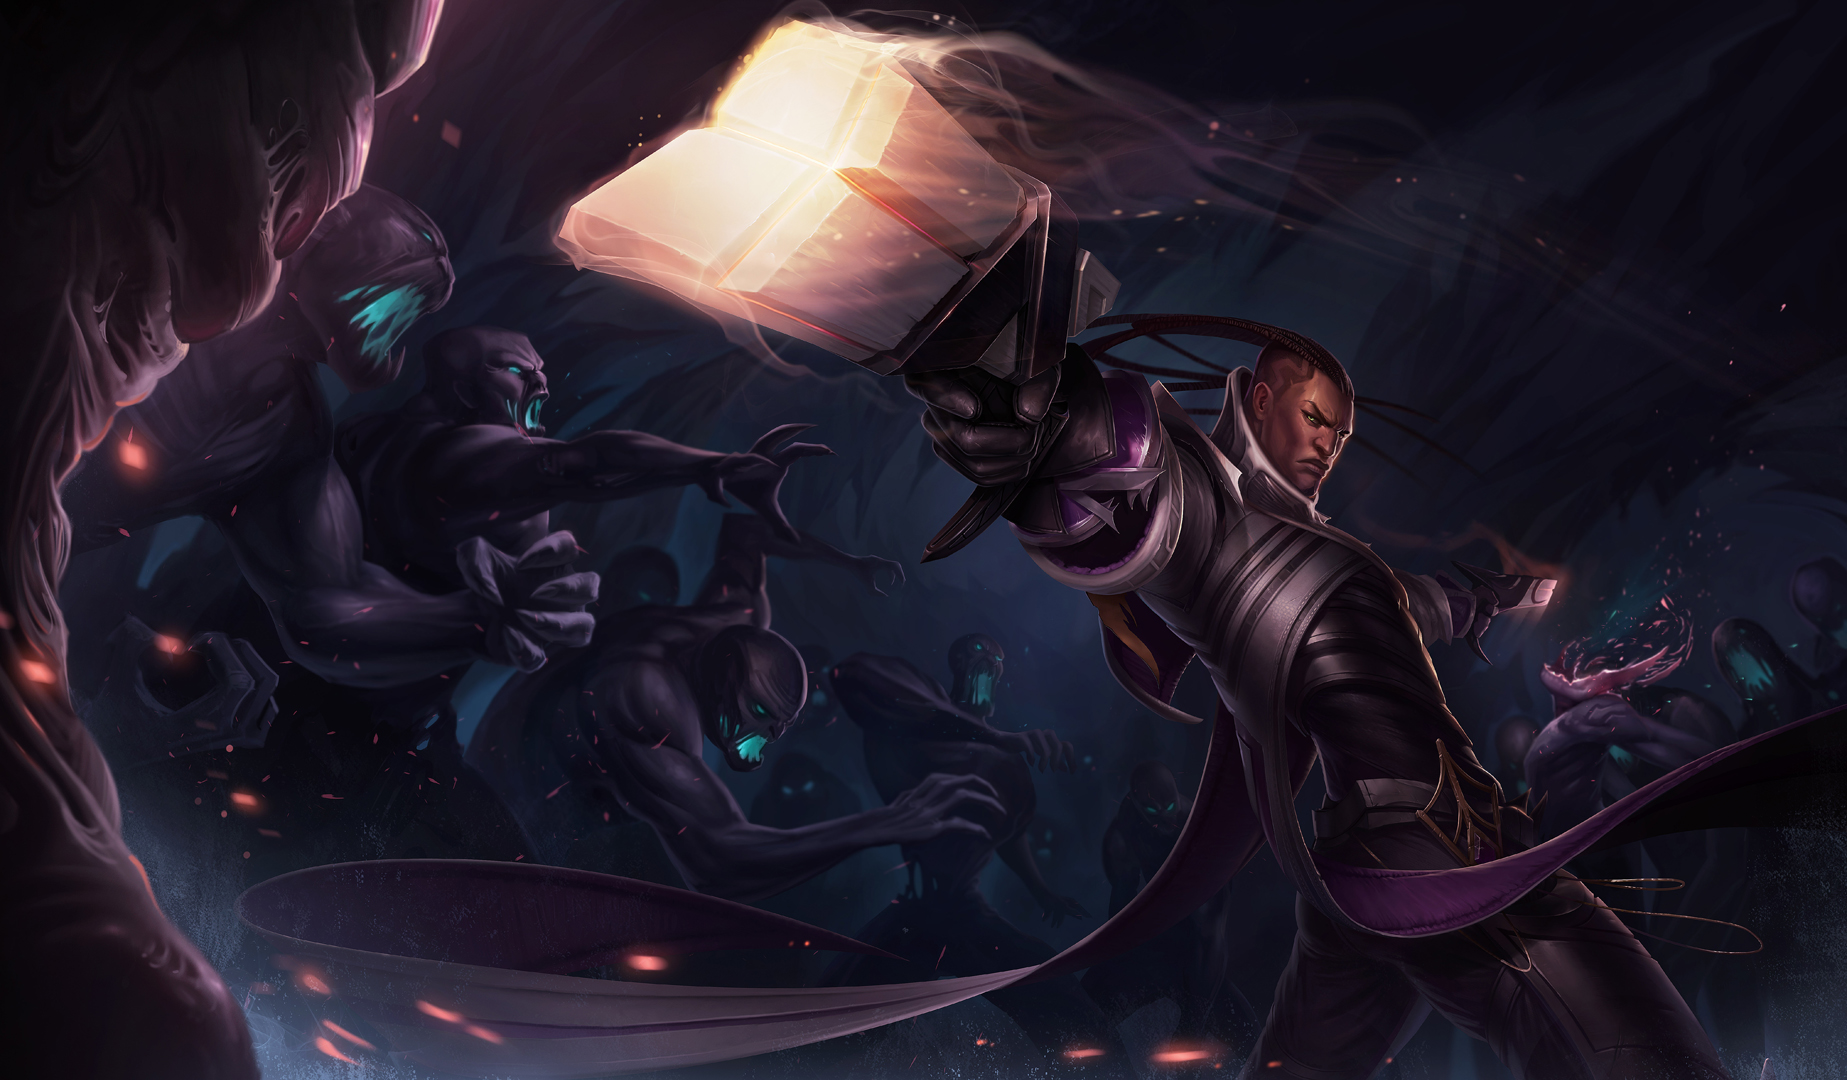
\includegraphics[scale = 0.1]{demo1_target_FFT.jpg}
		}
		\subfigure[outcome]{
			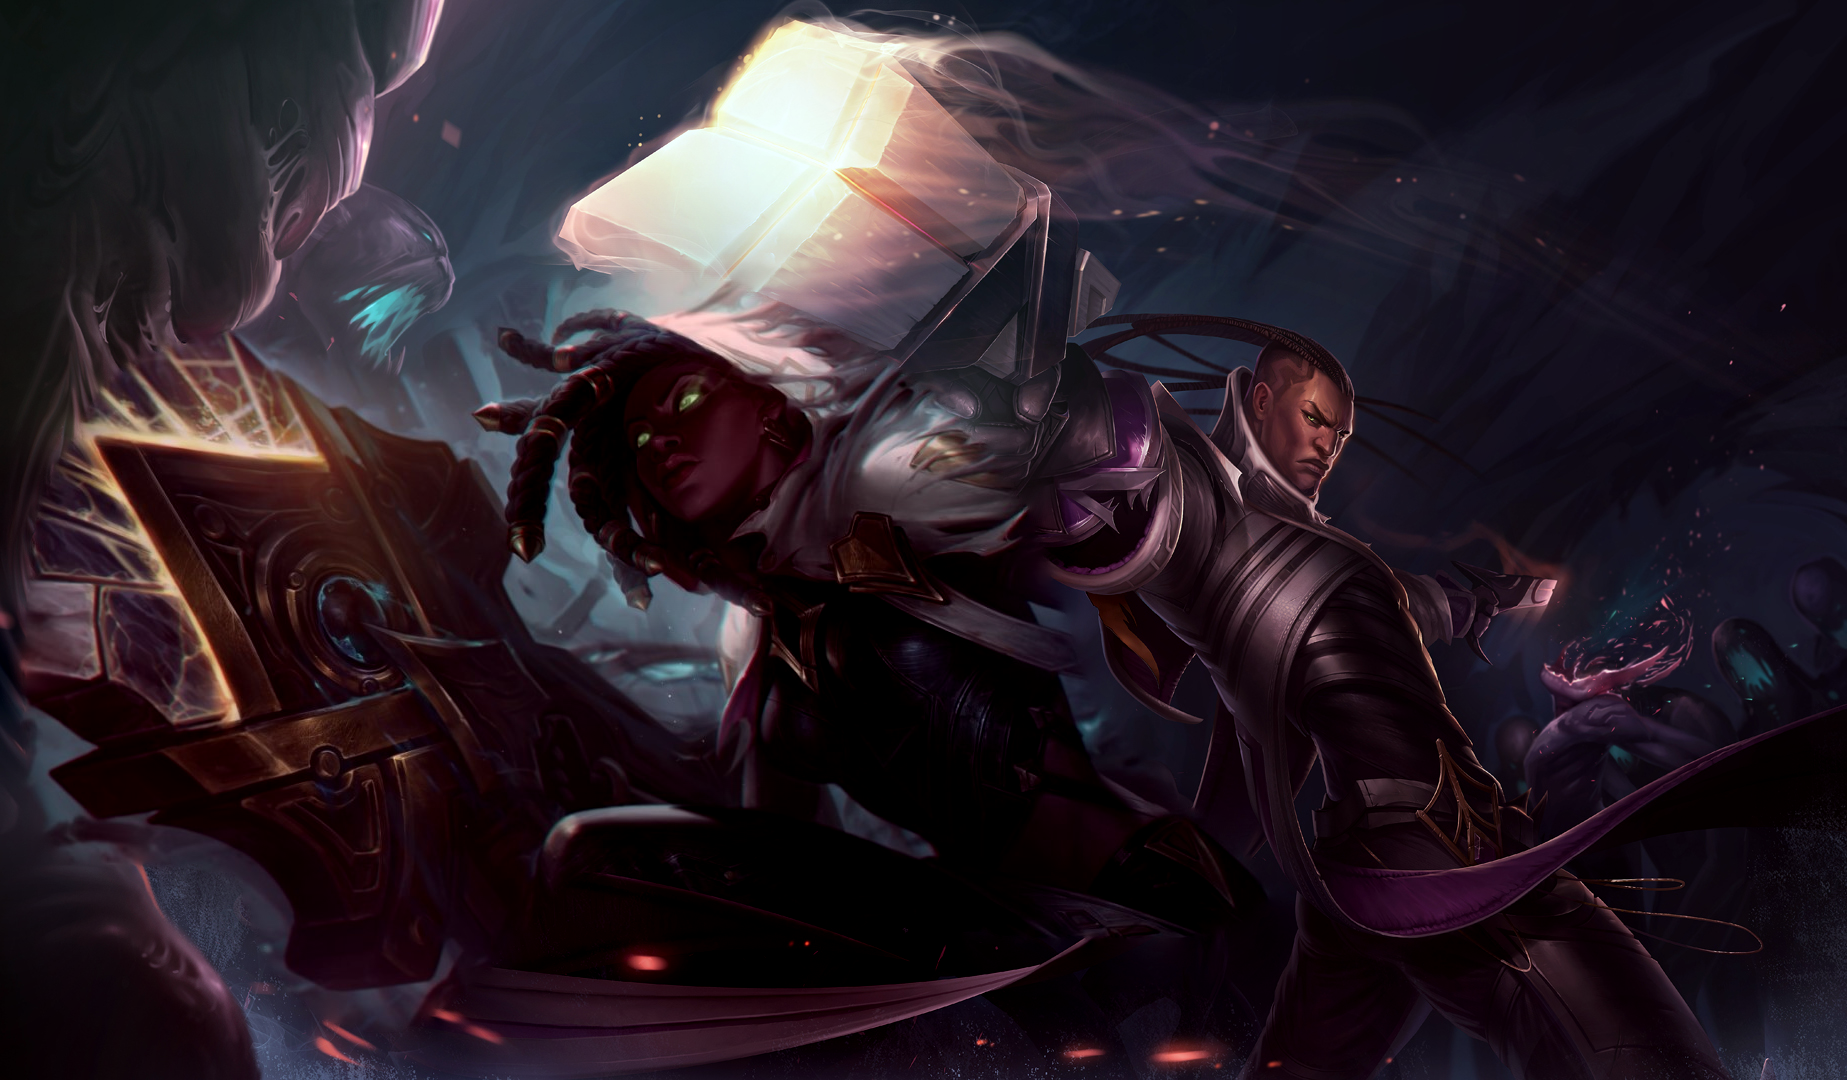
\includegraphics[scale = 0.1]{demo1_outcome_FFT.png}
		}
		\caption{Importing gradients}
	\end{figure}
	
	\begin{figure}[H]
		\centering
		\subfigure[source]{
			\includegraphics[scale=0.1]{demo5_sources_FFT.jpg}
		}
		\subfigure[mask]{
			\includegraphics[scale = 0.1]{demo5_mask_FFT.jpg}
		}
		
		\subfigure[target]{
			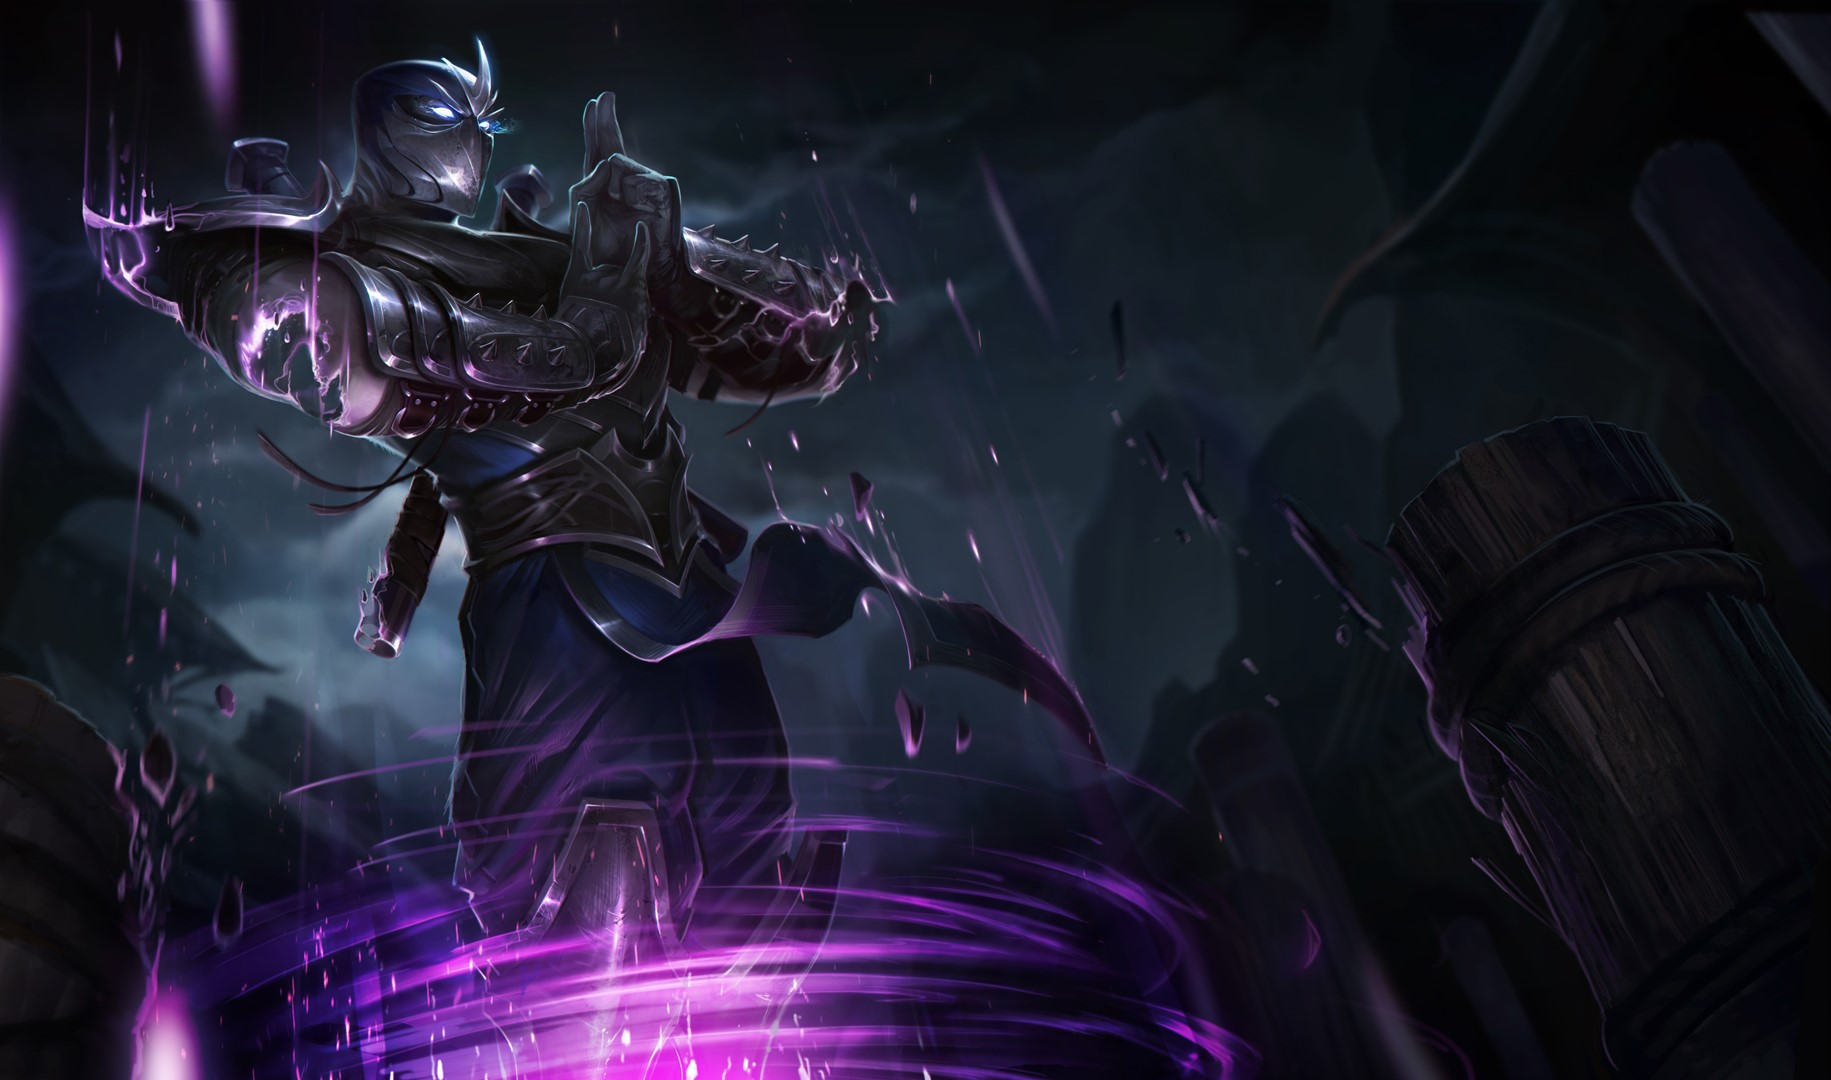
\includegraphics[scale = 0.1]{demo5_target_FFT.jpg}
		}
		\subfigure[outcome]{
			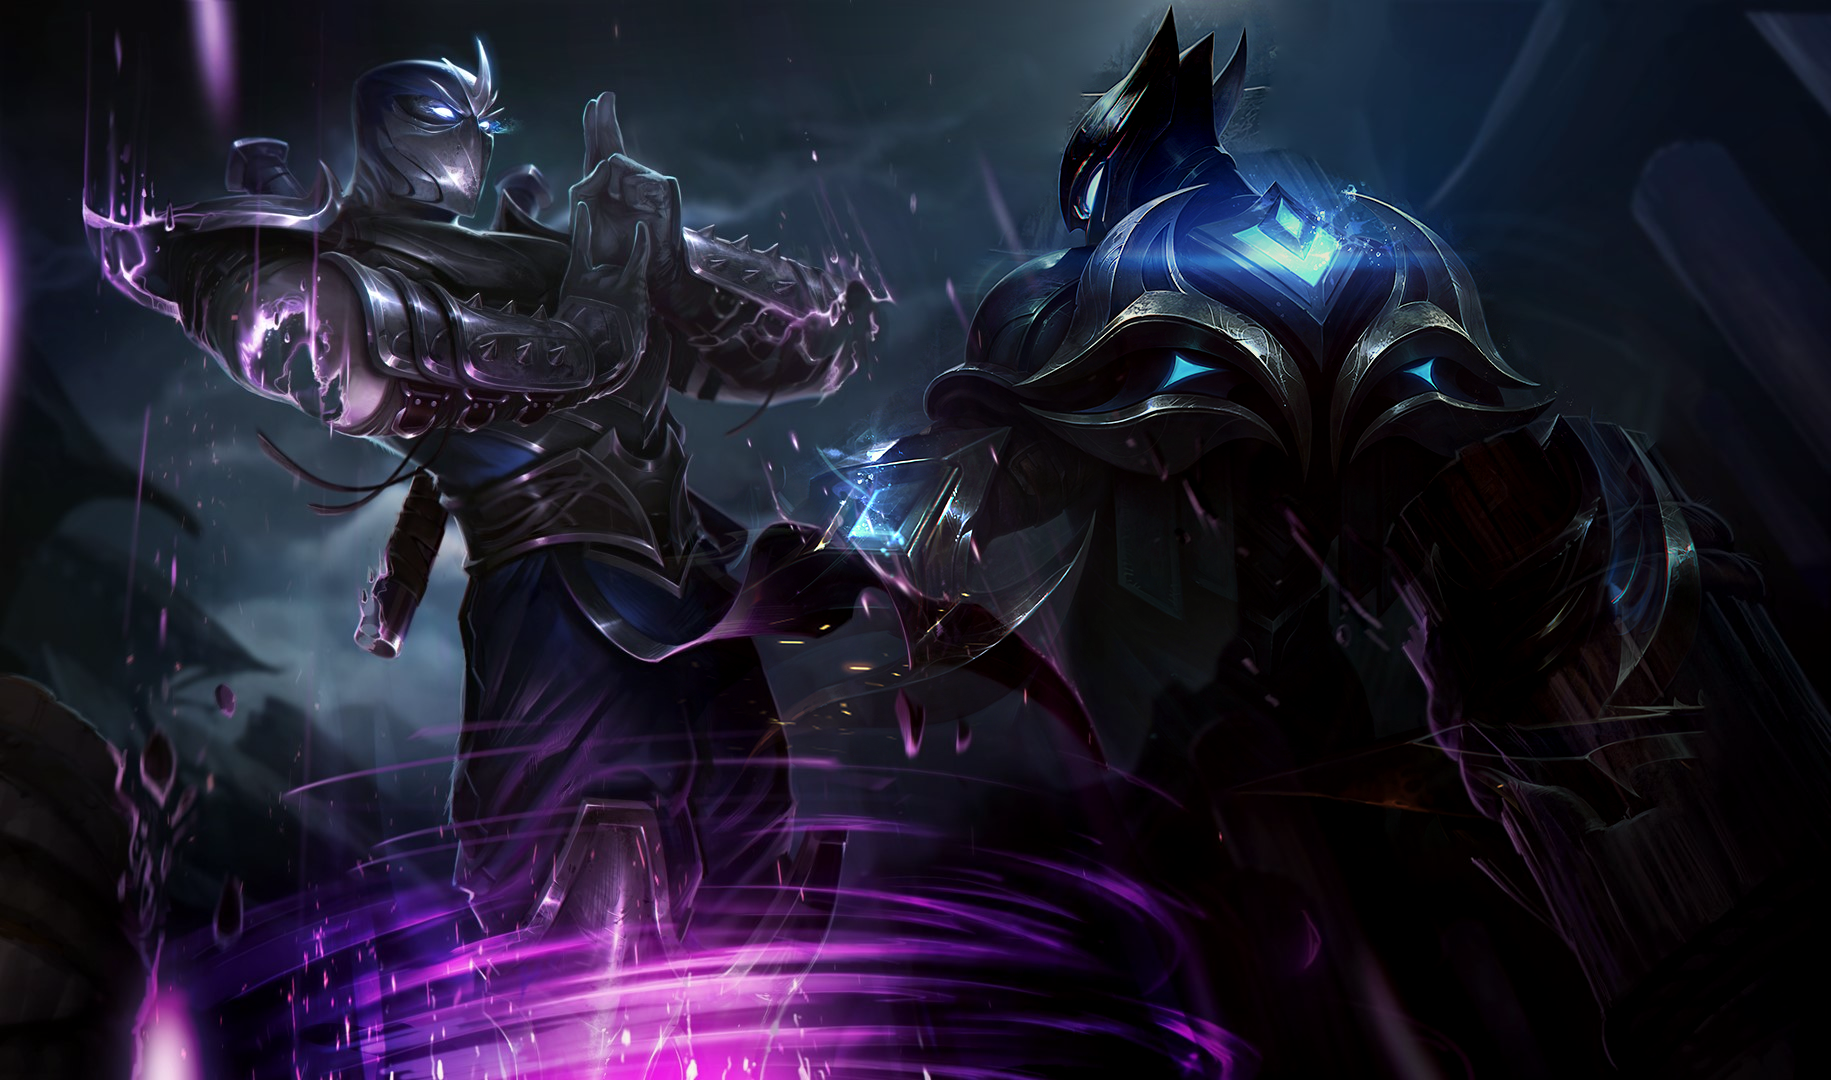
\includegraphics[scale = 0.1]{demo5_mixed_outcome_FFT.png}
		}
		\caption{Mixing gradients}
	\end{figure}

\section{Algorithms}
	
	The following two pseudocodes are brief conclusion of my codes, for more details, just take a look at the directory "src".
	
	\begin{algorithm}[H]
		\caption{Poisson image editing with FDM}
		\renewcommand{\algorithmicrequire}{\textbf{Input:}}
		\renewcommand{\algorithmicensure}{\textbf{Output:}}
		\renewcommand{\algorithmicreturn}{\textbf{Return:}}
		\begin{algorithmic}[1]
			\REQUIRE source image, target image, mask image, rectangular domain $\Omega$, location
			\ENSURE interpolated image
			\FOR{pixels in $\Omega$}
				\IF{the pixel is not being masked by mask image}
					\STATE Compute the gradient using the information of source image(importing gradients) or Compute the gradient using the information of both source and target image and pick the one with largest length(Mixing gradients)
				\ENDIF
			\ENDFOR
			\STATE Solve the poisson equation on the given $\Omega$ using Gauss-Seidel iteration
			\RETURN the interpolated image
		\end{algorithmic}
	\end{algorithm}
	
	\begin{algorithm}[H]
		\caption{Poisson image editing with FFT}
		\renewcommand{\algorithmicrequire}{\textbf{Input:}}
		\renewcommand{\algorithmicensure}{\textbf{Output:}}
		\renewcommand{\algorithmicreturn}{\textbf{Return:}}
		\begin{algorithmic}[1]
			\REQUIRE source image, target image, mask image, rectangular domain $\Omega$, location
			\ENSURE interpolated image
			\FOR{pixels in the entire domain}
				\IF{the pixel is not inside $\Omega$}
					\STATE Compute the gradient using the information of target image
				\ELSE
					\IF{the pixel is not being masked by the mask image}
						\STATE Compute the gradient using the information of source image(importing gradients) or Compute the gradient using the information of both source and target image and pick the one with largest length(Mixing gradients)
					\ELSE
						Compute the gradient using the information of target image
					\ENDIF
				\ENDIF
			\ENDFOR
			\STATE extend the gradient fields to make it antisymmetric
			\STATE compute the DFT of extended $f$ entry-wisly using the equation (13) and set the zero frequency as 0
			\STATE compute extended $f$ through inverse Fourier transformation, compute the gap between average value of the target image and average value of the solution(outside of $\Omega$), then shift the solution by this gap.
			\RETURN the interpolated image
		\end{algorithmic}
	\end{algorithm}

\section{Conclusion}
	
	The poisson image editing is sometimes a useful and funny ways to interpolate part of a image to another one, which gives a good way to recreate images. During the implementation of this project, I learnt new ideas for solving the poisson equations on a given domain and have so much fun creating lots of wierd(sometimes unbelievable) images. Feel free to check the directory "image" to see demos of my project. But apart from all the good things, we could still see that the approach sometimes leads to bad image quality. There are also some incompletion parts of my job, such as the Gauss-Seidel solver I wrote is not that efficent, the interfaces of my function are not that perfect, the codes I wrote are not that fluent and easy to understand.
	
	\begin{figure}[H]
		\centering
		\subfigure[source]{
			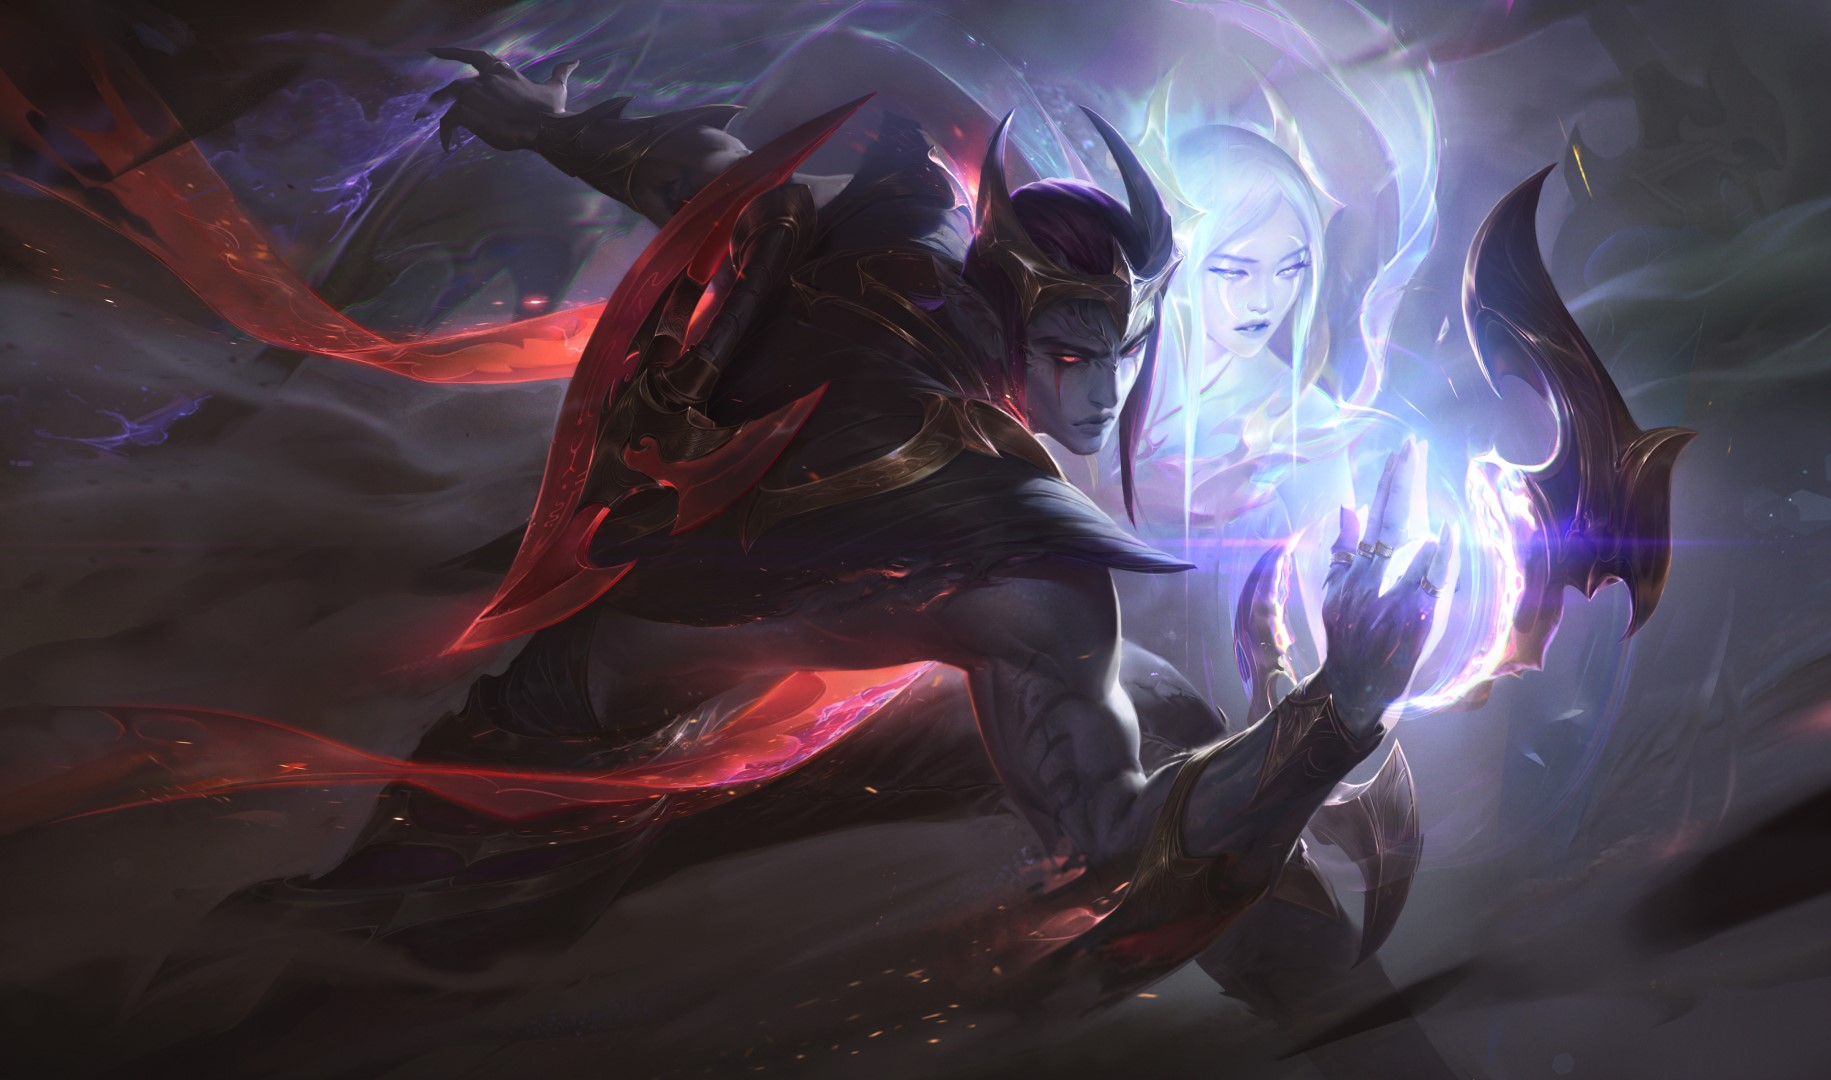
\includegraphics[scale=0.1]{demo2_sources_FFT.jpg}
		}
		\subfigure[mask]{
			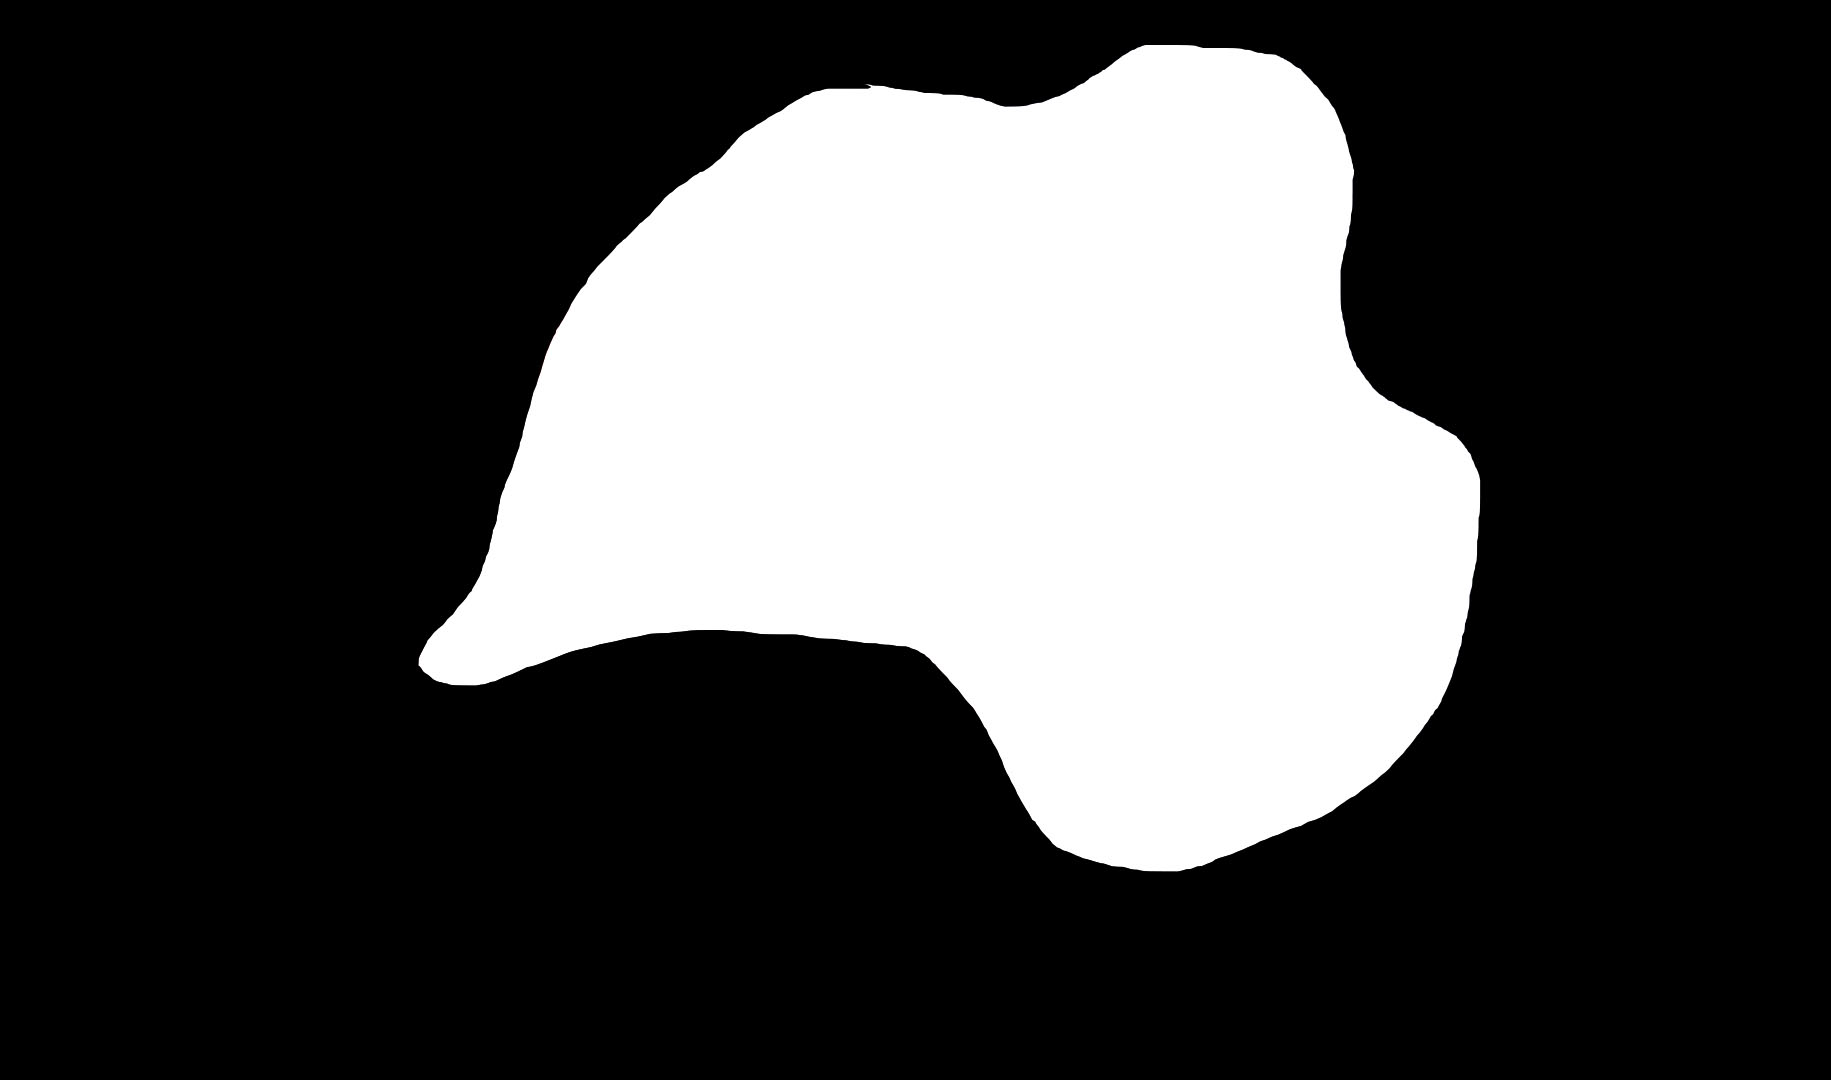
\includegraphics[scale = 0.1]{demo2_mask_FFT.jpg}
		}
		
		\subfigure[target]{
			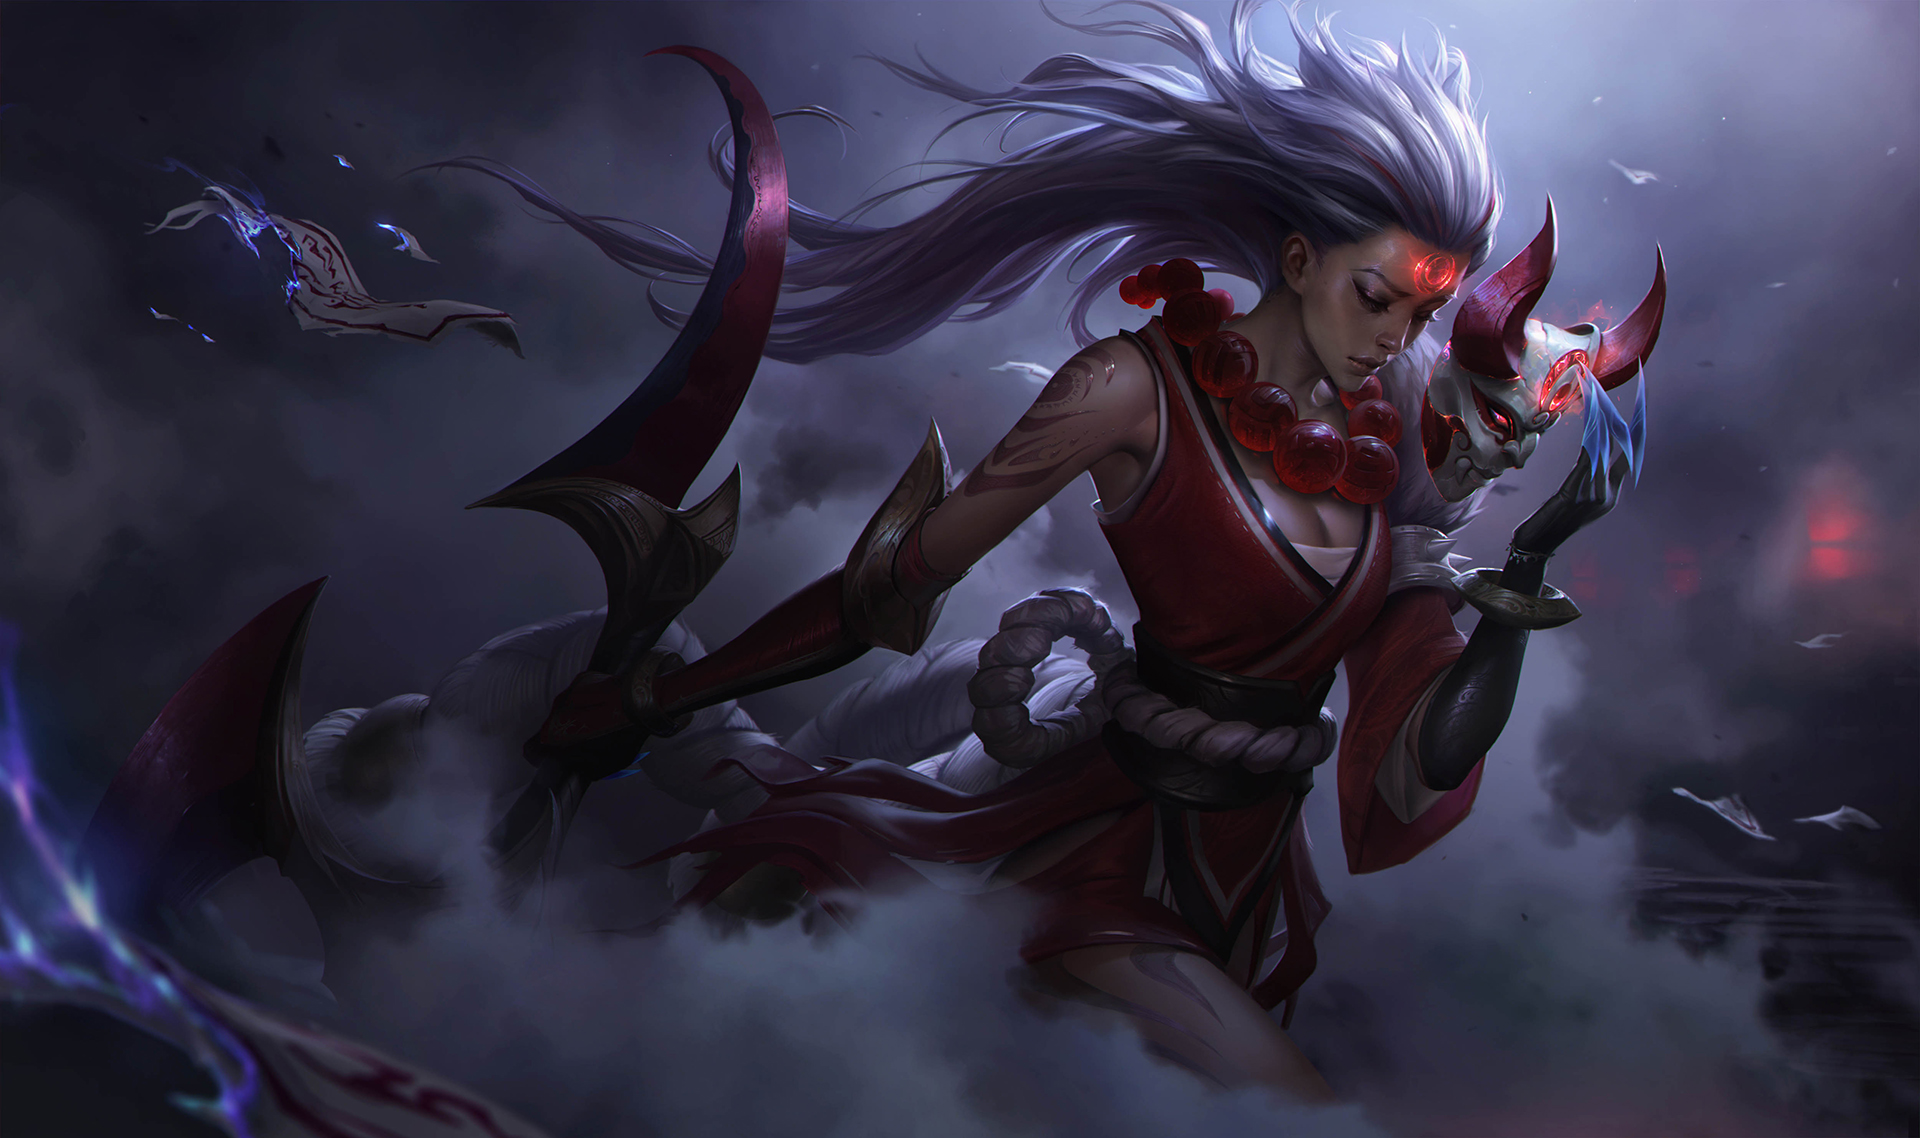
\includegraphics[scale = 0.1]{demo2_target_FFT.jpg}
		}
		\subfigure[outcome]{
			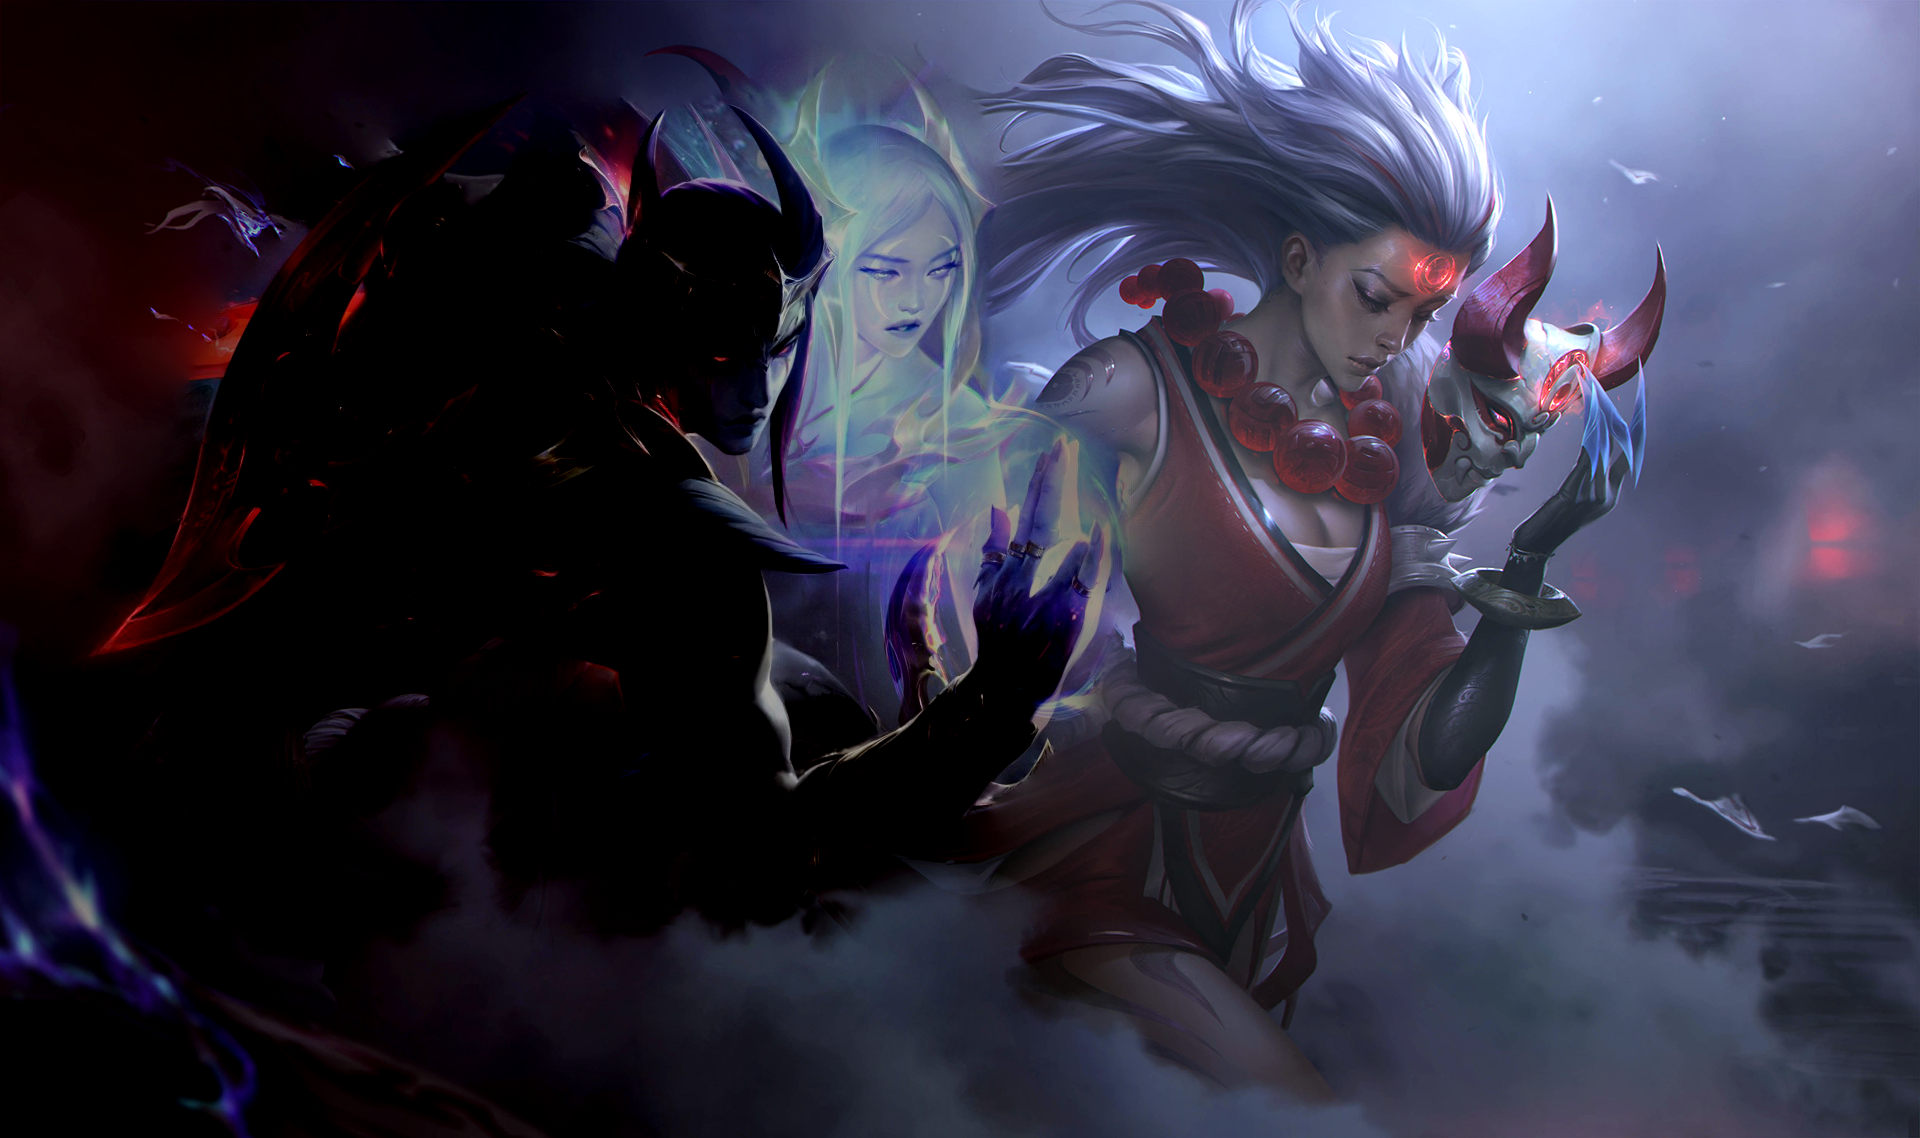
\includegraphics[scale = 0.1]{demo2_outcome_FFT.png}
		}
		\caption{A case that the interpolant becomes too dark that it is hard to see the details of it. I guess the problem is the drastic brightness difference between selected area and outside the area of the target image. Moreover, the lack of brightness of the source image might also contributes to the bad quality.}
	\end{figure}
	

\section{References}
	
	$\left[1\right]$ P. P\'erez, M. Gangnet, and A. Blake, \textit{Poisson image editing}, ACM Transactions on Graphics, 22 (2003), p.314-318.
	~\\
	$\left[2\right]$ J. Mat\'ias Di Martino, Gabriele Facciolo, Enric Meinhardt-Llois, \textit{Poisson Image Editing}, Image Processing On Line, 6 (2016), p.300-325.
	~\\
	$\left[3\right]$ http://cs.brown.edu/courses/csci1950-g/results/proj2/pdoran/
	~\\
	$\left[4\right]$ https://www.ipol.im/pub/art/2016/163/?utm\_source=doi
\end{document}


